\documentclass{beamer}

\beamertemplatenavigationsymbolsempty

\title{Polyhedral design\\with blended $n$-sided interpolants}
\author{P\'eter Salvi}
\institute{Budapest University of Technology and Economics}
\date{GrafGeo'24\\\vspace{1em}Budapest, April 10--11, 2024}

\begin{document}

\begin{frame}
  \titlepage
\end{frame}

\begin{frame}
  \frametitle{Outline}
  \hfill\includegraphics[width=.35\textwidth]{images/face-gradient.png}\\
  \vspace{-10em}
  \tableofcontents
  \centering
  \includegraphics[height=2.5em]{images/iit.png}$\qquad$
  \includegraphics[height=3em]{images/bme.jpg}
\end{frame}

\section{General idea}

\begin{frame}
  \frametitle{Construction plan}
  \centering
  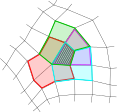
\includegraphics[width=.7\textwidth]{images/idea.pdf}
\end{frame}

\begin{frame}
  \frametitle{Interpolant \#1}
  \centering
  \includegraphics[width=.6\textwidth]{images/blend1.pdf}
\end{frame}

\begin{frame}
  \frametitle{Interpolant \#2}
  \centering
  \includegraphics[width=.6\textwidth]{images/blend2.pdf}
\end{frame}

\begin{frame}
  \frametitle{Interpolant \#3}
  \centering
  \includegraphics[width=.6\textwidth]{images/blend3.pdf}
\end{frame}

\begin{frame}
  \frametitle{Interpolant \#4}
  \centering
  \includegraphics[width=.6\textwidth]{images/blend4.pdf}
\end{frame}

\begin{frame}
  \frametitle{Blended patch}
  \centering
  \includegraphics[width=.6\textwidth]{images/blend5.pdf}
\end{frame}

\AtBeginSection[]{
 \begin{frame}
   \frametitle{Outline}
   \tableofcontents[currentsection]
 \end{frame}
}

\section{Regular meshes}

\subsection{Quadratic B\'ezier patches}

\begin{frame}
  \frametitle{Quadratic B\'ezier patches}
  \begin{columns}   
    \column{0.5\textwidth}
    \centering
    
\includegraphics[width=\textwidth]{images/qb.pdf}
    \column{0.5\textwidth}
    \[\mathbf{I}(u,v)=\sum_{i=0}^{2}\sum_{j=0}^{2}\mathbf{P}_{ij}B_{i}^{2}(u)B_{j}^{2}(v)\]
    \[\begin{aligned}
      \mathbf{P}_{02}&=\mathbf{C}_{2}&\mathbf{P}_{12}&=\hat{\mathbf{E}}_{2}&\mathbf{P}_{22}&=\mathbf{C}_{1}\\
      \mathbf{P}_{01}&=\hat{\mathbf{E}}_{3}&&&\mathbf{P}_{21}&=\hat{\mathbf{E}}_{1}\\
      \mathbf{P}_{00}&=\mathbf{C}_{3}&\mathbf{P}_{10}&=\hat{\mathbf{E}}_{4}&\mathbf{P}_{20}&=\mathbf{C}_{4}
    \end{aligned}\]
    \[\hat{\mathbf{E}}_{i}=2\mathbf{E}_{i}-\frac{1}{2}(\mathbf{C}_{i-1}+\mathbf{C}_{i})\]
    \[\mathbf{P}_{11}=\frac{1}{4}(16\mathbf{M}-\sum_{i=1}^{4}(\mathbf{C}_{i}+2\hat{\mathbf{E}}_{i}))\]
  \end{columns}
  \[[0,1]^2\rightarrow[0.5,1]^2\quad\Rightarrow\quad\mathbf{S}(0,0)=\mathbf{M},\ \ \mathbf{S}(1,1)=\mathbf{C}_{1},\text{etc.}\]
\end{frame}

\begin{frame}
  \frametitle{Patch equation}
  \[\mathbf{S}(u,v)=\sum_{i=1}^{4}\mathbf{I}_{i}\left(\frac{u_{i}+1}{2},\frac{v_{i}+1}{2}\right)\Phi(u_{i},v_{i})\]
  Local parameterization:
  \begin{columns}   
    \column{0.7\textwidth}
    \[
    \begin{aligned}
      u_{1}&=u&v_{1}&=v\\
      u_{2}&=v&v_{2}&=1-u\\
      u_{3}&=1-u&v_{3}&=1-v\\
      u_{4}&=1-v&v_{4}&=u
    \end{aligned}
    \]
    \column{0.3\textwidth}
    \centering
    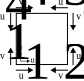
\includegraphics[width=.9\textwidth]{images/param4.pdf}
  \end{columns}
  Blends:
  \[\Phi(u,v)=\Psi(u)\cdot\Psi(v)\]
  \[\begin{aligned}
  \Psi(0)&=1&\Psi(1)&=0&\Psi^{(k)}(0)&=\Psi^{(k)}(1)=0
  \end{aligned}\]
  \centering (for some $k>0$)
\end{frame}

\subsection{Blending functions}

\begin{frame}
  \frametitle{Blending functions}
  $G^k$ Hermite blend: $\Psi(t)=\sum_{i=0}^{k}B_{i}^{2k+1}(t)$
  \centering
  \includegraphics[width=.9\textwidth]{images/blend-functions.pdf}
\end{frame}

\section{Irregular vertices}

\subsection{Quadratic Generalized B\'ezier (QGB) patches}

\begin{frame}
  \frametitle{Quadratic Generalized B\'ezier patches -- Parameterization}
  \begin{itemize}
  \item Regular domain: $\{(\cos\frac{2k\pi}{n},\sin\frac{2k\pi}{n})\}$, $k=0\dots n-1$
  \item Wachspress coordinate-based local parameters:
  \[\begin{aligned}
  s_{i}(u,v)&=\lambda_{i}/(\lambda_{i-1}+\lambda_{i}),&d_{i}(u,v)&=1-\lambda_{i-1}-\lambda_{i}
  \end{aligned}\]
  \end{itemize}
  \includegraphics[width=.45\textwidth]{images/wachspress.pdf}\hfill
  \includegraphics[width=.45\textwidth]{images/sh-parameters.pdf}\\\vspace{1em}
\end{frame}

\begin{frame}
  \frametitle{Quadratic Generalized B\'ezier patches -- Equation}
  \vspace{-1em}
  \[\!\!\!\!\!\!
    \mathbf{I}(u,v)=\sum_{i=1}^{n}\Bigg(\mathbf{C}_{i-1}\frac{1}{2}B_{0}^{2}(s_{i})+
    \hat{\mathbf{E}}_{i}B_{1}^{2}(s_{i})+
    \mathbf{C}_{i}\frac{1}{2}B_{2}^{2}(s_{i})\Bigg)B_{0}^{2}(d_{i})+
    \mathbf{P}_{0}B_{0}(u,v)\]
  \begin{columns}   
    \column{0.5\textwidth}
    \centering
    
\includegraphics[width=\textwidth]{images/qgb.pdf}
    \column{0.5\textwidth}
    \[\mathbf{P}_{0}=\frac{n^{2}\mathbf{M}-\sum_{i=1}^{n}\left(\mathbf{C}_{i}+2\hat{\mathbf{E}}_{i}\right)}{n(n-3)}\]
    $B_{0}=$\\$\ \ 1-\sum_{i=1}^{n}\left(\frac{1}{2}B_{0}^{2}+B_{1}^{2}+\frac{1}{2}B_{2}^{2}\right)B_{0}^{2}$
    \vspace{1em}
    \begin{itemize}
    \item $n=4\Rightarrow$ B\'ezier patch
    \item $n=3\Rightarrow$ B\'ezier triangle
    \end{itemize}
  \end{columns}
\end{frame}

\subsection{Parameterization}

\begin{frame}
  \frametitle{Parameter mapping -- Problem}
  \centering
  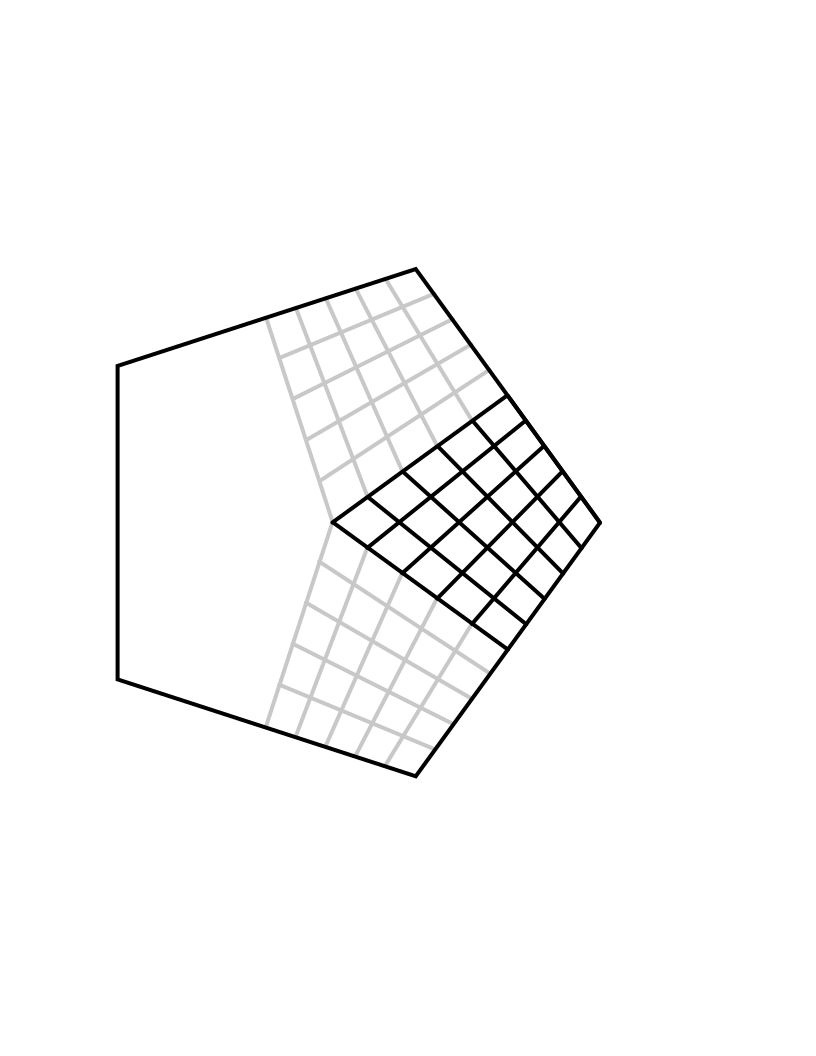
\includegraphics[width=.7\textwidth]{images/bilinear-multi.pdf}
\end{frame}

\begin{frame}
  \frametitle{Parameter mapping -- Solution}
  \begin{columns}   
    \column{0.65\textwidth}
    \begin{itemize}
    \item Rational B\'ezier curves:
      \[\mathbf{r}(t)=\frac{\sum_{i=0}^{2}\mathbf{R}_{i}w_{i}B_{i}^{2}(t)}{\sum_{i=0}^{2}w_{i}B_{i}^{2}(t)}\]
    \item Central weight: $1/u$
    \item Control points:
      \[\begin{aligned}
      \mathbf{R}_{0}&=\mathbf{V}_{0}(1-u)+\mathbf{V}_{1}u\\
      \mathbf{R}_{1}&=\mathbf{V}_{2}u\cdot e^{u(u-1)}\\
      \mathbf{R}_{2}&=\mathbf{V}_{4}(1-u)+\mathbf{V}_{3}u
      \end{aligned}\]
    \item Intersection with golden section search
    \end{itemize}
    \column{0.35\textwidth}
    \centering
    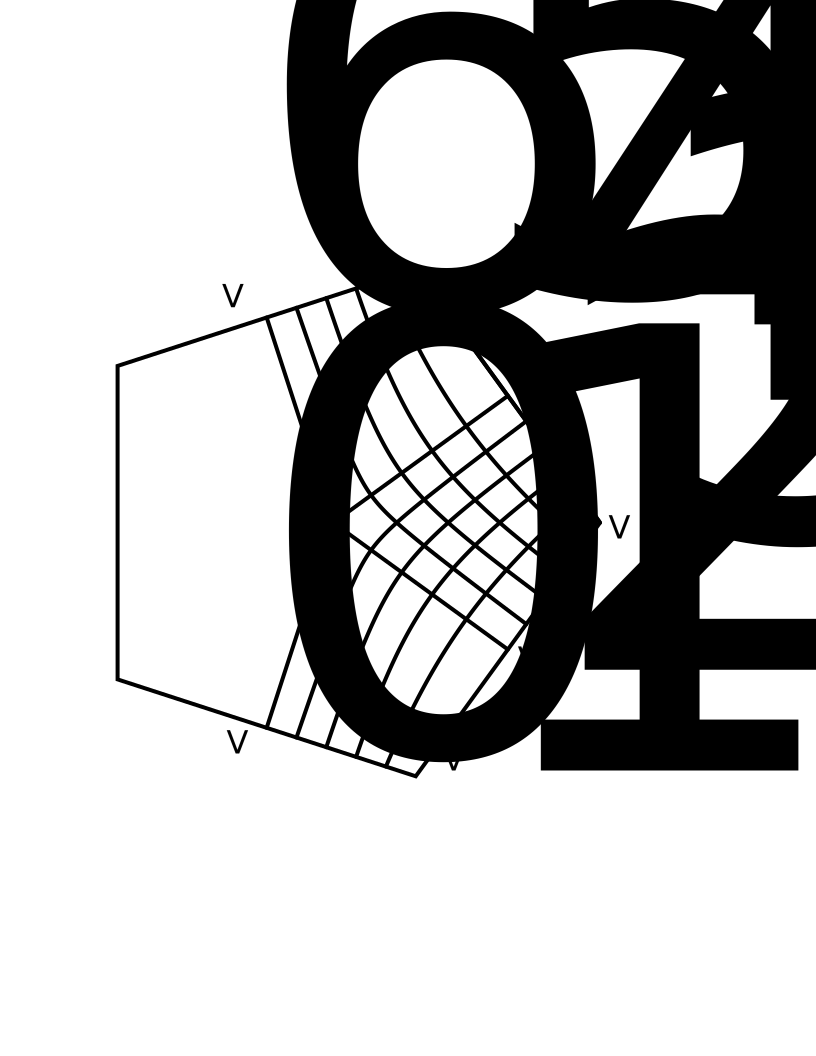
\includegraphics[width=\textwidth]{images/rational.pdf}\vspace{1em}
    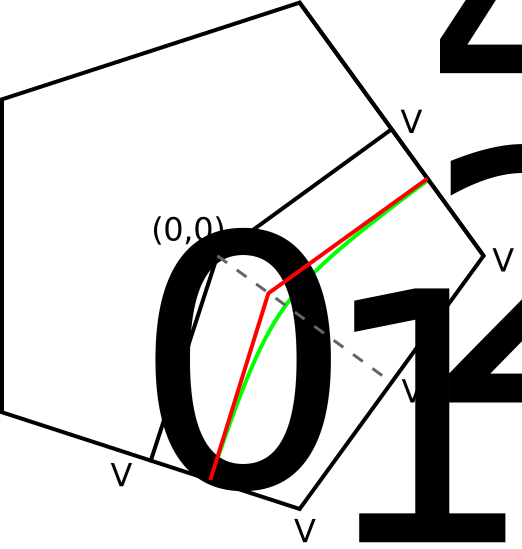
\includegraphics[width=\textwidth]{images/rational-control.pdf}
  \end{columns}
\end{frame}

\begin{frame}
  \frametitle{Parameter mapping -- Concave case}
  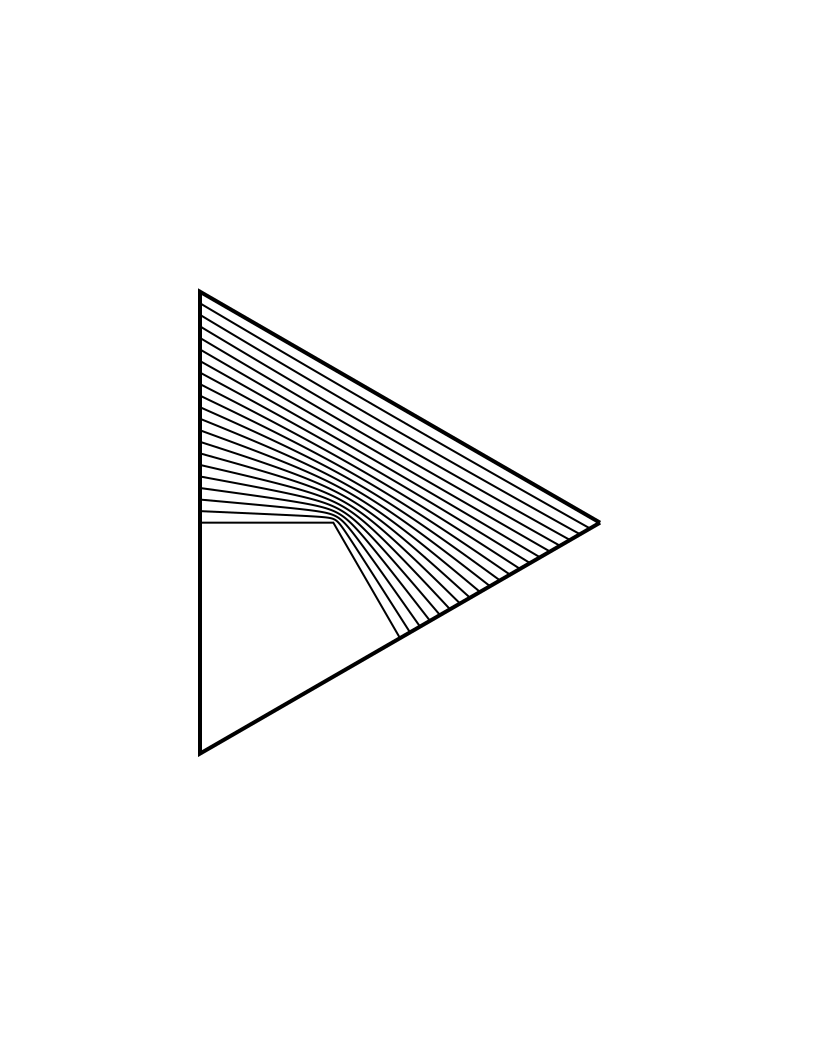
\includegraphics[width=.6\textwidth]{images/rational3.pdf}
  \centering
\end{frame}

\subsection{Triangular patches}

\begin{frame}
  \frametitle{Triangular patches}
  \begin{itemize}
  \item Triangular QGB patch $\equiv$ quadratic B\'ezier triangle
  \item $\rightarrow$ no central control $\Rightarrow$ elevate to cubic:
  \end{itemize}
  \vspace{1em}
  \[\mathbf{I}(u,v)=\sum_{i+j+k=3}\mathbf{P}_{ijk}\frac{6}{i!j!k!}\lambda_{1}^{i}\lambda_{2}^{j}\lambda_{3}^{k}\]
  where
  \[\begin{aligned}
  \mathbf{P}_{300}&=\mathbf{C}_{1},\quad\mathbf{P}_{030}=\mathbf{C}_{2},\quad\mathbf{P}_{003}=\mathbf{C}_{3},\\\mathbf{P}_{210}&=\frac{1}{3}(\mathbf{C}_{1}+2\hat{\mathbf{E}}_{2}),\quad\mathbf{P}_{120}=\frac{1}{3}(\mathbf{C}_{2}+2\hat{\mathbf{E}}_{2}),\\\mathbf{P}_{021}&=\frac{1}{3}(\mathbf{C}_{2}+2\hat{\mathbf{E}}_{3}),\quad\mathbf{P}_{012}=\frac{1}{3}(\mathbf{C}_{3}+2\hat{\mathbf{E}}_{3}),\\\mathbf{P}_{102}&=\frac{1}{3}(\mathbf{C}_{3}+2\hat{\mathbf{E}}_{1}),\quad\mathbf{P}_{201}=\frac{1}{3}(\mathbf{C}_{1}+2\hat{\mathbf{E}}_{1}),\\
  \mathbf{P}_{111}&=\frac{1}{6}(27\mathbf{M}-\sum_{\max(i,j,k)=3}\mathbf{P}_{ijk}-3\sum_{\max(i,j,k)=2}\mathbf{P}_{ijk})
  \end{aligned}\]
\end{frame}

\section{Results}

\begin{frame}
  \frametitle{Trebol model -- Cage}
  \centering
  \includegraphics[width=.7\textwidth]{images/trebol-cage.png}
\end{frame}

\begin{frame}
  \frametitle{Trebol model -- Isophotes}
  \centering
  \includegraphics[width=.7\textwidth]{images/trebol-iso.png}
\end{frame}

\begin{frame}
  \frametitle{Trebol model -- Mean curvature}
  \centering
  \includegraphics[width=.7\textwidth]{images/trebol-mean.png}
\end{frame}

\begin{frame}
  \frametitle{Torus model -- Cage}
  \centering
  \includegraphics[width=.85\textwidth]{images/torus-cage.png}
\end{frame}

\begin{frame}
  \frametitle{Torus model -- Isophotes}
  \centering
  \includegraphics[width=.85\textwidth]{images/torus.png}
\end{frame}

\begin{frame}
  \frametitle{Icosahedron model -- Cage}
  \centering
  \includegraphics[width=.6\textwidth]{images/icosahedron-cage.png}
\end{frame}

\begin{frame}
  \frametitle{Icosahedron model -- Cage after 1 Catmull--Clark step}
  \centering
  \includegraphics[width=.6\textwidth]{images/icosahedron-cage-cc.png}
\end{frame}

\begin{frame}
  \frametitle{Icosahedron model -- Mean curvature}
  \centering
  \includegraphics[width=.6\textwidth]{images/icosahedron-mean.png}
\end{frame}

\begin{frame}
  \frametitle{Duck model -- Cage \& surface}
  \centering
  \includegraphics[width=.85\textwidth]{images/bob-surf.png}
\end{frame}

\begin{frame}
  \frametitle{Duck model -- Slicing}
  \centering
  \includegraphics[width=.85\textwidth]{images/bob-slicing.png}
\end{frame}

\begin{frame}
  \frametitle{Duck model -- Mean curvature}
  \centering
  \includegraphics[width=.85\textwidth]{images/bob-mean.png}
\end{frame}

\begin{frame}
  \frametitle{Conclusions \& future work}
  \begin{columns}   
    \column{0.5\textwidth}
    \begin{itemize}
    \item Parametric surface
    \item Interpolates mesh vertices of arbitrary topology
    \item Meshes with boundary?
    \item Continuous boundary constraints?
    \item Shape parameters?
    \item Normal vector interpolation?
    \end{itemize}
    \column{0.5\textwidth}
    \centering
    \includegraphics[width=\textwidth]{images/bob-env.png}
  \end{columns}
  \vspace{1em}
  \centering
  \includegraphics[height=4em]{images/qrcode.pdf}\\
  \texttt{https://3dgeo.iit.bme.hu/}
\end{frame}

\end{document}
